\subsection{Preprocessing}
\label{subsec:prepro}
The proposed preprocessing steps for the MRIs consist of bias correction using the N4ITK algorithm \cite{n4itk}, followed by image normalization to an interval of [0,1], automatic selection of a region of interest (ROI), image re-sampling, and contour interpolation.  

The ROI, containing the prostate gland, is automatically obtained from the intersection of the rectangular prisms of the three MRI planes \cite{anneke}. The ROI is re-sampled to a resolution of $0.5 \times 0.5 \times 0.5$ mm  using linear interpolation \cite{itk}. Finally, after the images are cropped and resampled, they are linearly interpolated to an isotropic volume with a resolution of $168^3$. Figure \ref{fig_1} shows an example of the resulting 2D slice of a T2-w MRI after being preprocessed.
%\begin{figure}[h]
%    \centering
%    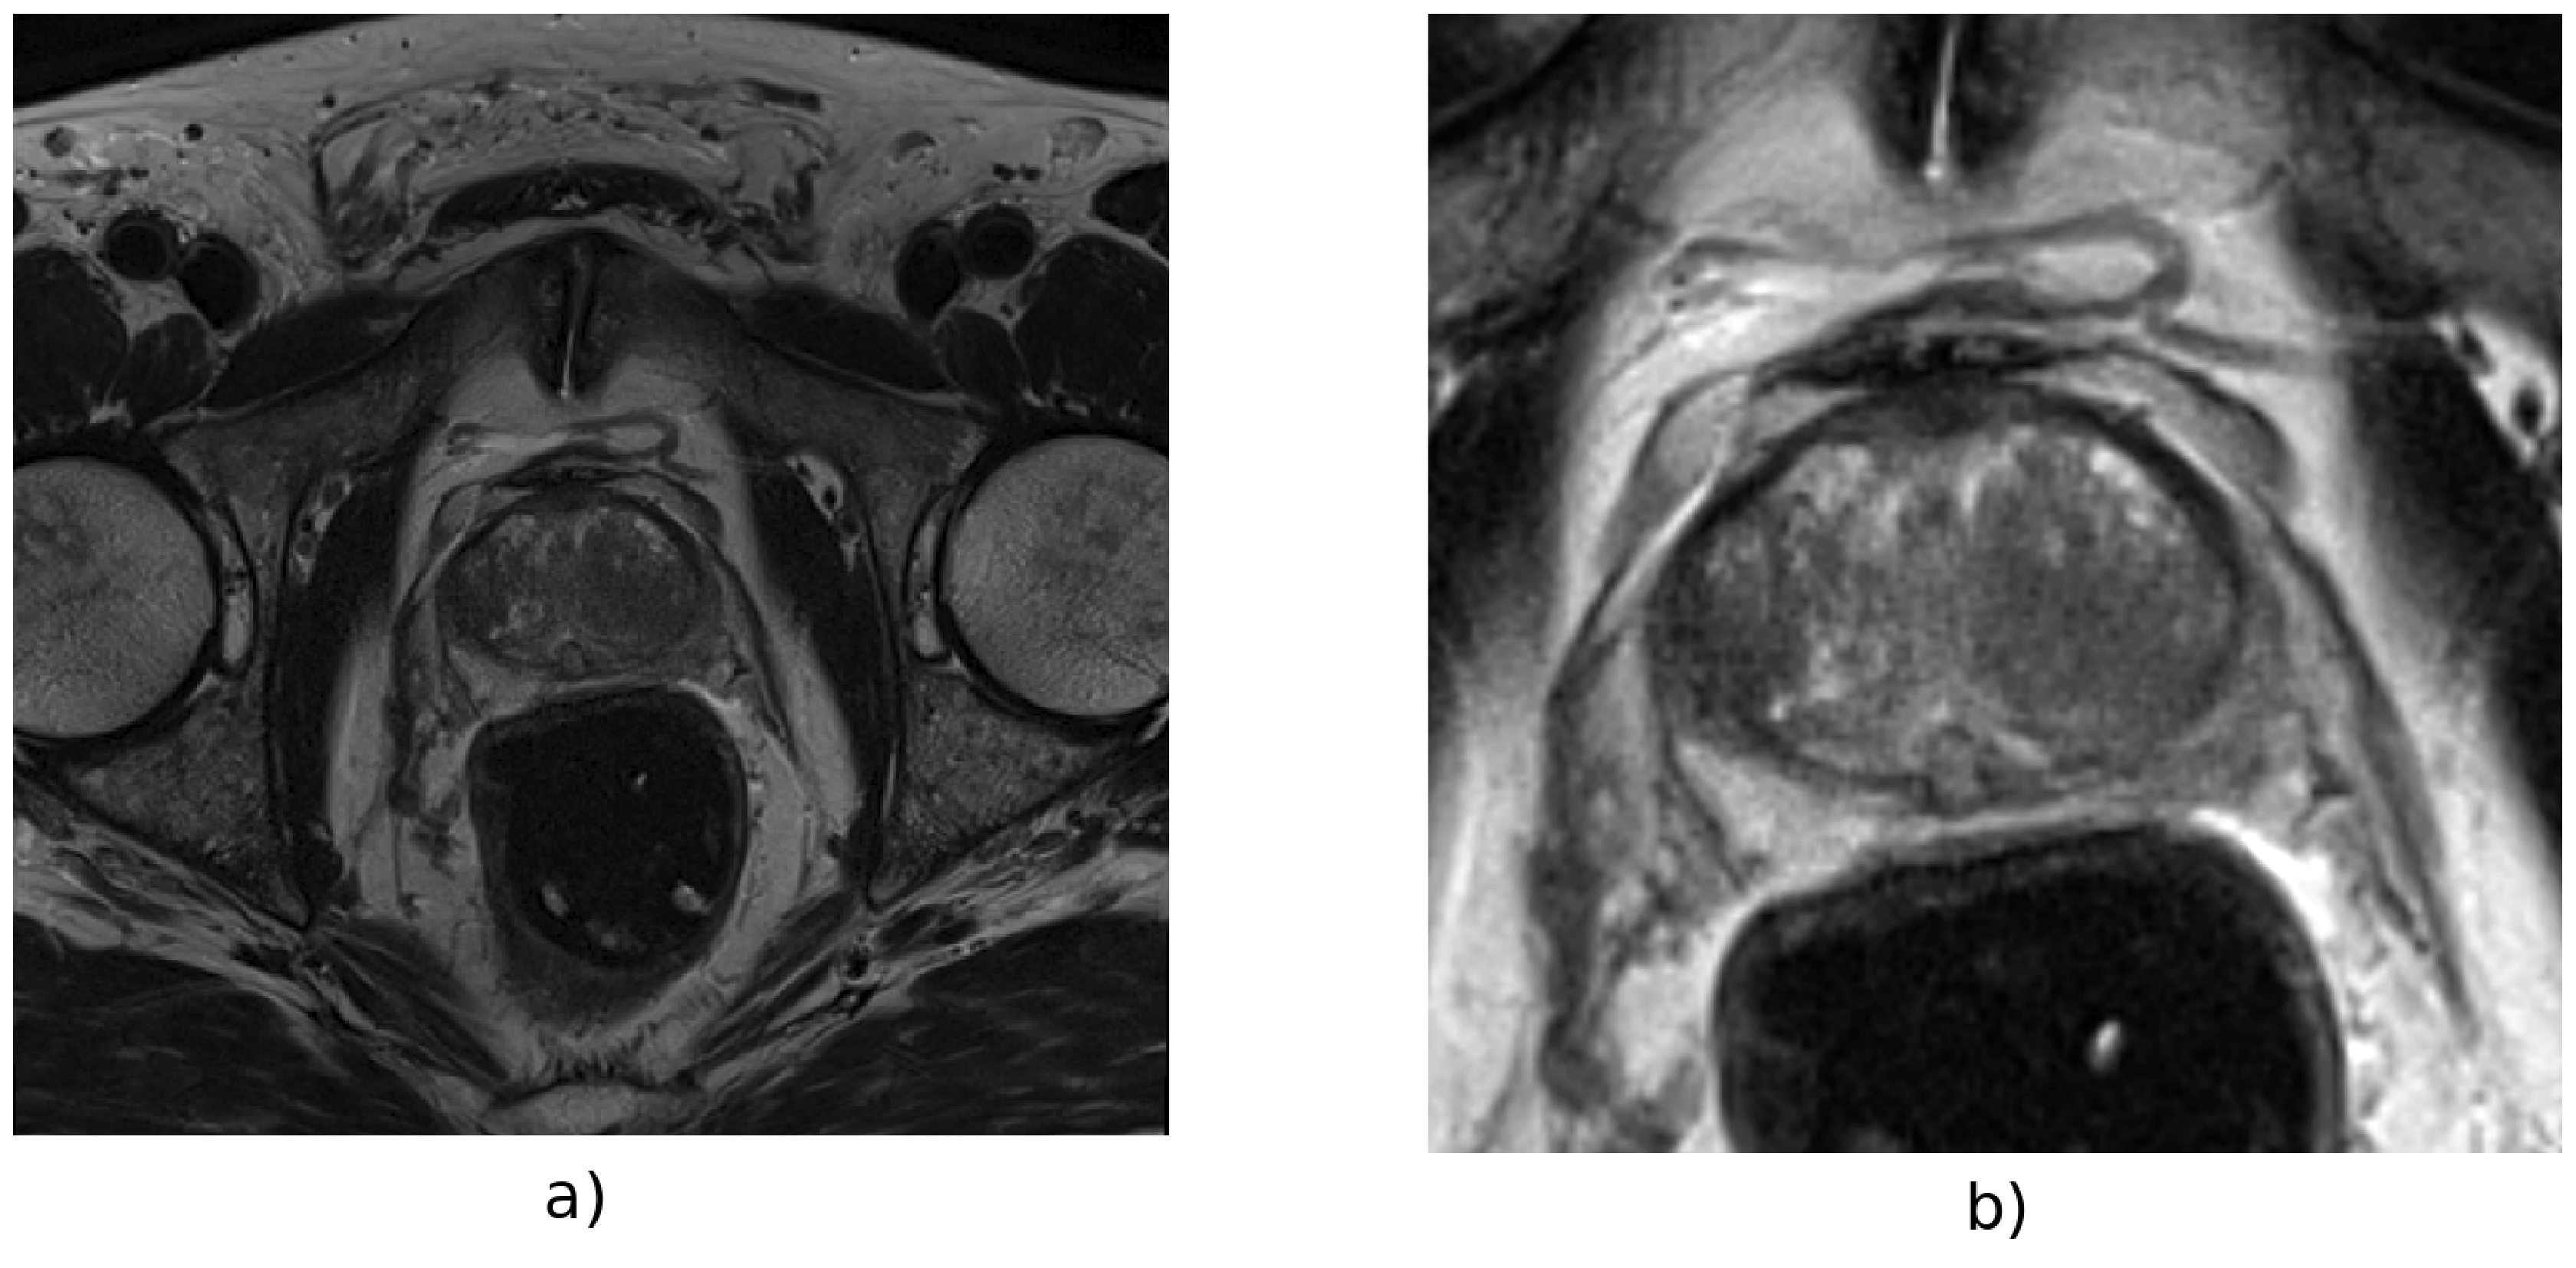
\includegraphics[totalheight=.25\textheight]{figures/Figure1.eps}
%    \caption{The MRIs are preprocessed with bias correction, normalization, resampling, and cropped to a ROI to reduce the variability of sizes and intensities between magnets. In this example, \textbf{a)} is the original image and \textbf{b)} is the image after being processed.} 
%    \label{fig_1}
%\end{figure}

Contour preprocessing included interpolation using optical flow.  The manual contours were carried out on the original T2-w MRI resolution and hence the necessity for interpolation. The proposed method estimates 2D contours in-between slices of the axial plane and computes them independently for every two consecutive slices. First, optical flow is obtained between the two contours of adjacent slices using the Farneback method \cite{optflow}. Then, intermediate contours are generated by linearly interpolating the position of their edges following the direction of the optical flow vector field. Figure \ref{fig:fig_2} shows an example of the optical flow obtained between two horizontal slices and the resulting interpolated 3D volume using this method. 
%\begin{figure}[h]
%    \centering
%    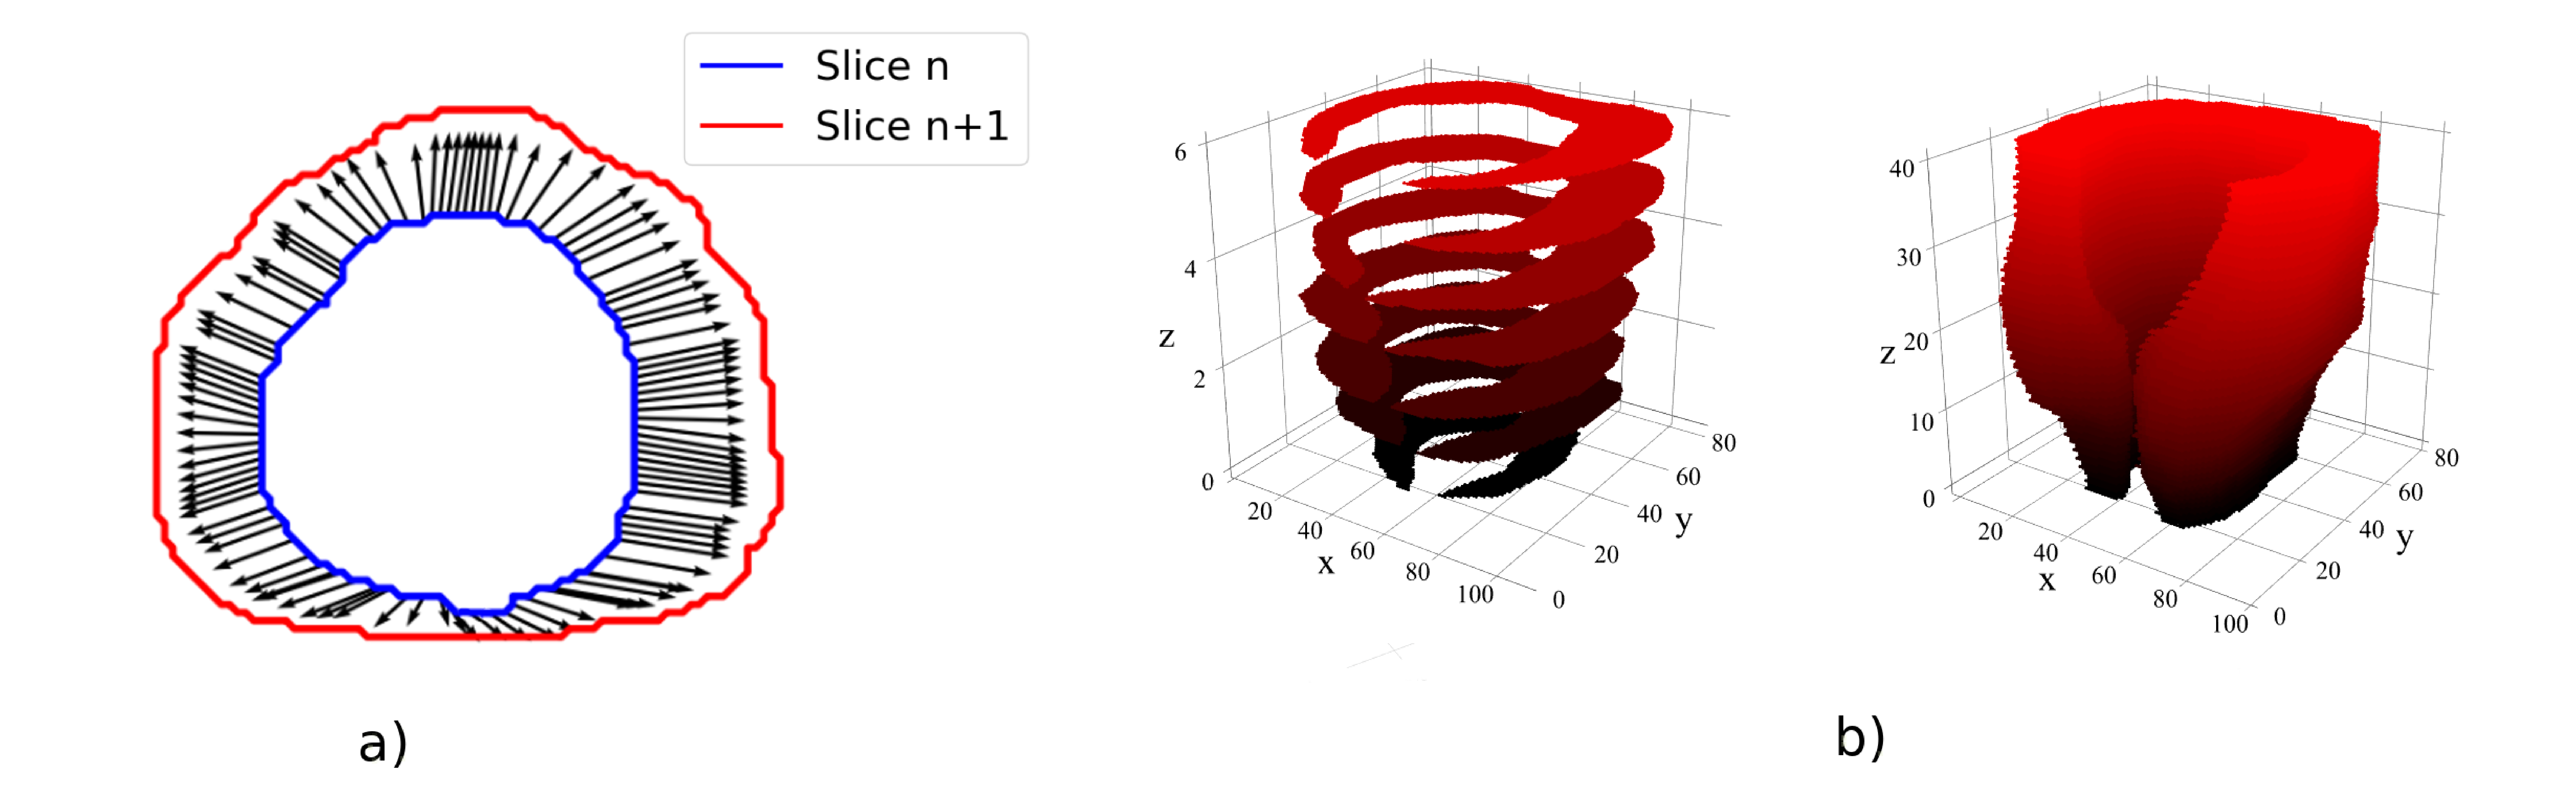
\includegraphics[totalheight=.21\textheight]{figures/Figure2.eps}
%    \caption{Example of the proposed algorithm to increase the resolution of prostate and PZ contours. In \textbf{a)}, an example of the optical flow obtained between two prostate contours from adjacent horizontal planes. In \textbf{b)} on the left, original contours with 17 slices. On the right, interpolated contours with 68 slices.}
%    \label{fig:fig_2}
%\end{figure}

